\chapter{Improving Non-factoid Question Answering}
\label{chapter:non-factoid}

Factoid questions studied in Chapter~\ref{chapter:factoid} represent only a fraction of user information needs, and there are many other types of questions, which cannot be answered with entity names or dates.
The variety of user information needs is reflected in different types of questions, that people post to community question answering websites~\cite{harper2010question,ignatova2009annotating,Liu:2008:USA:1599081.1599144}.
Such questions usually require a longer response, \eg a paragraph of text, list of instructions, \etc
For the majority of such questions, modern search engines still return the ``10 blue links'', and delegate the task of digging into the information and extracting relevant pieces of knowledge to the user, which can be quite time-consuming.
In this Chapter, I focus on improving question answering for such generic information needs.

Previous research on non-factoid question answering either focused on a small subset of questions (\eg definition questions~\cite{hildebrandt2004answering}), or considered this as a problem of ranking existing answers in CQA archives, which can be reused to answer new questions~\cite{carmel2000eresponder,Shtok:2012:LPA:2187836.2187939}.
To advance the research in the area of automatic question answering for a general class of user information needs in 2015 TREC started a series of LiveQA evaluation campaigns\footnote{\href{url}{http://trec-liveqa.org}}.
The TREC LiveQA track task is to develop a real-time system to answer real user questions, that are posted live to Yahoo!~Answers\footnote{\href{url}{http://answers.yahoo.com/}} community question answering platform.

This chapter describes the methods and ideas I implemented in a system, that participated in 2015 and 2016 versions of the track.
The system uses a combination of semi-structured information, \ie question-answer pairs from different CQA platforms, with unstructured information, which can be extracted from regular web documents.
The former strategy of retrieving similar previously posted questions was shown to be quite effective~\cite{carmel2000eresponder,Shtok:2012:LPA:2187836.2187939}, as it allows a system to return a naturally looking answer in cases when a good match was found.
However, many similar questions are formulated differently, which complicates the retrieval problem, additionally, many incoming information needs are still unique and there are simply no similar questions in the archive.
In this case a system can extract its answer from potentially relevant passages of regular web documents.
In Section~\ref{section:non-factoid:system} I will describe the architecture of \textit{EmoryQA}: the system I developed to participate in the TREC LiveQA shared task.

Despite the indisputable improvements in automatic answer selection\footnote{\href{url}{http://aclweb.org/aclwiki/index.php?title=Question\_Answering\_(State\_of\_the\_art)}}, the analysis of results of TREC LiveQA 2015 task demonstrated, that we still have a big gap in performance between human and automatic question answering.
Mistakes, that were made by trained machine learning models for answer passage selection, could be easily spotted by a human in fractions of a second even when a person does not have enough expertise in the area of the question.
To build on this observation, we looked into how an automatic system can integrate crowdsourcing to improve its performance.
More specifically, we propose to use feedback of a crowd of workers to extend the answers pool and obtain quality labels for generated answer candidates.
Section~\ref{section:non-factoid:crowdsourcing} describes the design of the crowdsourcing component and the results of TREC LiveQA 2016, which demonstrated its effectiveness for near real-time question answering.

In summary, the main contributions of this chapter include:
\begin{itemize}
\item An open-source state-of-the-art automatic question answering system for a general class of user information needs, evaluated at TREC LiveQA 2015 and 2016 tracks.
The architecture of the system and evaluation results were published in TREC conference proceedings~\cite{savenkov2015trec,savenkov2016trec}.
\item A novel hybrid question answering system, that incorporates a crowdsourcing module, but still operates in near real-time, and significantly improves performance over the pure automatic approach.
This work was presented as a full paper at HCOMP 2016~\cite{savenkov_crqa2016}.
\end{itemize}

% -=-=-=-=-=-=-=-=-=-=-=-= LiveQA : Begin -=-=-=-=-=-=-=-=-=-=-=
\section{Ranking Answers and Web Passages for Non-factoid Question Answering}
\label{section:non-factoid:system}

In this section, I describe the architecture of \textit{EmoryQA} (Figure~\ref{figure:non-factoid:emoryqa}), the automatic question answering system, which combines semi-structured data from CQA archives and unstructured web document passages to cover a variety of questions that users have.

\begin{figure}
    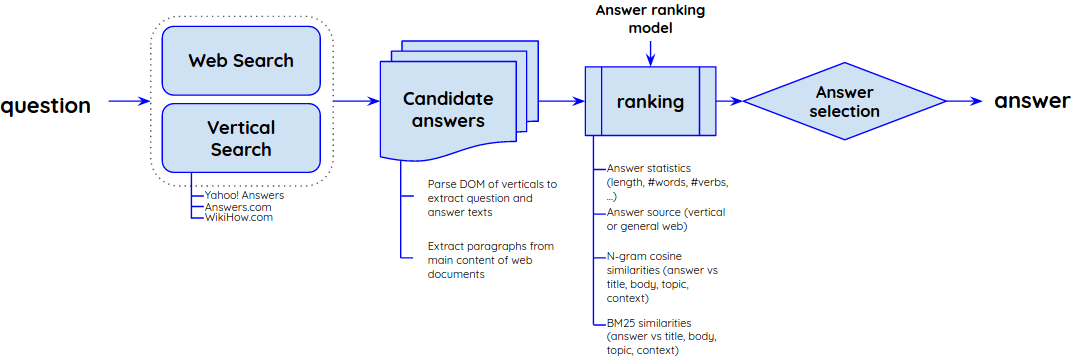
\includegraphics[width=\textwidth]{img/emoryqa_design}
    \caption{Architecture of the EmoryQA non-factoid question answering system, participated in TREC LiveQA shared task.}
    \label{figure:non-factoid:emoryqa}
\end{figure}

Community Question Answering websites became quite popular and millions of users post their questions there and hope to receive a response from the community.
The questions on these websites typically consist of question title, body, and category.
Since CQA archives accumulated a lot of question data, we chose this question format for our development, similar to the setup proposed for the TREC LiveQA shared task.
Below you can see an example question from a CQA website:

\begin{center}
\begin{tabular}{|p{12cm}|}
\hline
\textbf{Question category}: Astronomy \& Space\\
\textbf{Question title}: Why do people claim the Earth is not the center of the universe?\\
\textbf{Question body}: Clearly the sun and moon are moving around the Earth otherwise we would not have night and day.\\
\hline
\end{tabular}
\end{center}

People often have similar tasks and situations which pose the same questions, and therefore community question answering platforms receive many similar questions, which can be answered in a similar way.
Researchers have found out, that a good reply to similar questions can be reused to answer new user questions~\cite{carmel2000eresponder,Shtok:2012:LPA:2187836.2187939}, and a number of approaches have been proposed to rank candidate answer passages~\cite{fried2015higher,sharp2015spinning,soricut2006automatic,surdeanu2011learning,yang2016beyond}.
\textit{EmoryQA} builds on these works and includes components to retrieve a set of candidate answers from a number of community question answering platforms, such as Yahoo!~Answers~\footnote{\href{url}{http://answers.yahoo.com/}}, Answers.com~\footnote{\href{url}{http://answers.com/}} and WikiHow~\footnote{\href{url}{http://wikihow.com/}}.
Besides some frequent questions, there is always a long tail of requests, which are either unique or phrased differently from those that were previously submitted to a CQA website~\cite{bernstein2012direct}.
To help a user with such questions, \textit{EmoryQA} includes a general web search module, which extracts passages from regular web pages to extend the pool of candidate answers.

All candidate answers, extracted from either CQA verticals or regular web documents, are ranked together by a trained answer ranking model, and \textit{EmoryQA} returns the top scoring passage as the final answer to the question.
Next, we will describe candidate generation and ranking modules in more detail.

% ===========================================
\subsection{Candidate Answer Generation}
\label{section:non-factoid:system:candidates}

When the \textit{EmoryQA} system receives a user question, it first generates a set of candidate answers from CQA vertical and regular web search data sources.
User questions vary in language~\cite{AgichteinLG01} and the level of details, therefore to increase the recall and retrieve as many relevant results as possible, for each question we generate multiple search queries:
\begin{itemize}[itemsep=0em]
\item Question title, which most often captures the gist of the question
\item Two longest question sentences (detected by the presence of the question word at the beginning or question mark at the end of a sentence) from the title and body of the question. In some cases, the real user question is hidden inside the body, while the title just provides the overall topic of the question.
\item Concatenation of the question word, verbs and top-5 terms from the question title by inverse document frequency\footnote{IDF of terms are estimated using Google N-gram corpus: \href{url}{https://catalog.ldc.upenn.edu/LDC2006T13}}.
% This strategy targets over-specific questions, which often retrieve few if any search results.
\end{itemize}

For CQA verticals, \textit{EmoryQA} issues the queries to the built-in search interfaces of Yahoo!~Answers, Answers.com and WikiHow.com and extracts top-10 similar questions with the corresponding answers, posted by the community, and adds them to the candidates pool.
For regular web search, we rely on the Bing Web Search API\footnote{\href{url}{https://datamarket.azure.com/dataset/bing/searchweb}}, which we query to retrieve top-10 relevant documents and extract paragraphs of text from their main content, as detected by a method based on~\cite{Kohlschutter_2010}.

In addition to the candidate answers themselves, \textit{EmoryQA} extracts certain meta-data, that helps to estimate the relevance of a passage to the current question.
For regular web page paragraphs, it is useful to know the topic of the page (\eg its title) and the context (such as text that immediately precedes the paragraph in the document), as shown by Di Wang and Eric Nyberg in ~\cite{wang2015cmu}.
For CQA answers, our system stores the text of the corresponding question title, body, and category.
For convenience, we will refer to this question title and web page title as \textit{``answer topic''}, while the body of the retrieved question and the preceding text block for web candidates as \textit{``answer context''}.

% ===========================================
\subsection{Candidate ranking}
\label{section:non-factoid:system:ranking}

\textit{EmoryQA} represents each candidate answer with a set of features (Table~\ref{table:non-factoid:system:features}).
To predict the quality of the accumulated candidates and select the best answer we use a trained learning-to-rank model, which sorts the answers and selects the top response as the final answer to the question.
There are multiple ways to train such a ranking model depending on the type of data available.

\begin{table}[t]
\centering
\small
\begin{tabular}{p{13cm}}

\textbf{Answer statistics} \\
\hline
--- Length in chars, words and sentences \\
--- Average number of words per sentence \\
--- Fraction of non-alphanumeric characters  \\
--- Number of question marks \\
--- Number of verbs  \\
\hline
\textbf{Answer source} \\
\hline
--- Binary feature for each of the search verticals: Web, Yahoo! Answers, Answers.com, WikiHow.com \\
\hline
\textbf{N-gram matches}\\
\hline
--- Cosine similarities using uni-, bi- and tri-gram representations of the question title and/or body, and answer text, topic or context\\
--- The lengths of longest spans of matched terms between question title and/or body, and answer text, topic or context\\
\hline
\textbf{Information Retrieval score}\\
\hline
--- BM25 scores between question title and/or body, and answer text, topic or context\\ 
\end{tabular}
\caption{The list of candidate answer ranking features used by the EmoryQA non-factoid question answering system.}
\label{table:non-factoid:system:features}
\end{table}

% ------------------------------------------------
\subsubsection{Training answer ranking model using unlabeled CQA data}
\label{table:non-factoid:system:cqa_training}

The problem of learning to rank for information retrieval usually assumes the presence of labeled data, that provides some kind of partial order of documents for a set of queries~\cite{liu2009learning}.
For question answering that would mean that one needs to provide relevance labels for passages, which can be retrieved for a question.
This process is more expensive than for regular document search, since there are many more passages than documents, and a QA system is not even restricted to return a continuous text from a single document.

When no explicit labeled data is available, we can use implicit information available in CQA archives, \eg selected best answers.
The version of \textit{EmoryQA}, developed to participate in TREC LiveQA 2015, had two trained models: LSTM recurrent neural network based model, used as one of the features for the final logistic regression model that scores all candidates and selects the best one as the answer.
To train these models I used WebScope Yahoo!~Answers dataset\footnote{\href{url}{https://webscope.sandbox.yahoo.com/catalog.php?datatype=l}}, and the process of building the training datasets is explained on Figure~\ref{figure:non-factoid:system:model_training}.

\begin{figure}[t]
    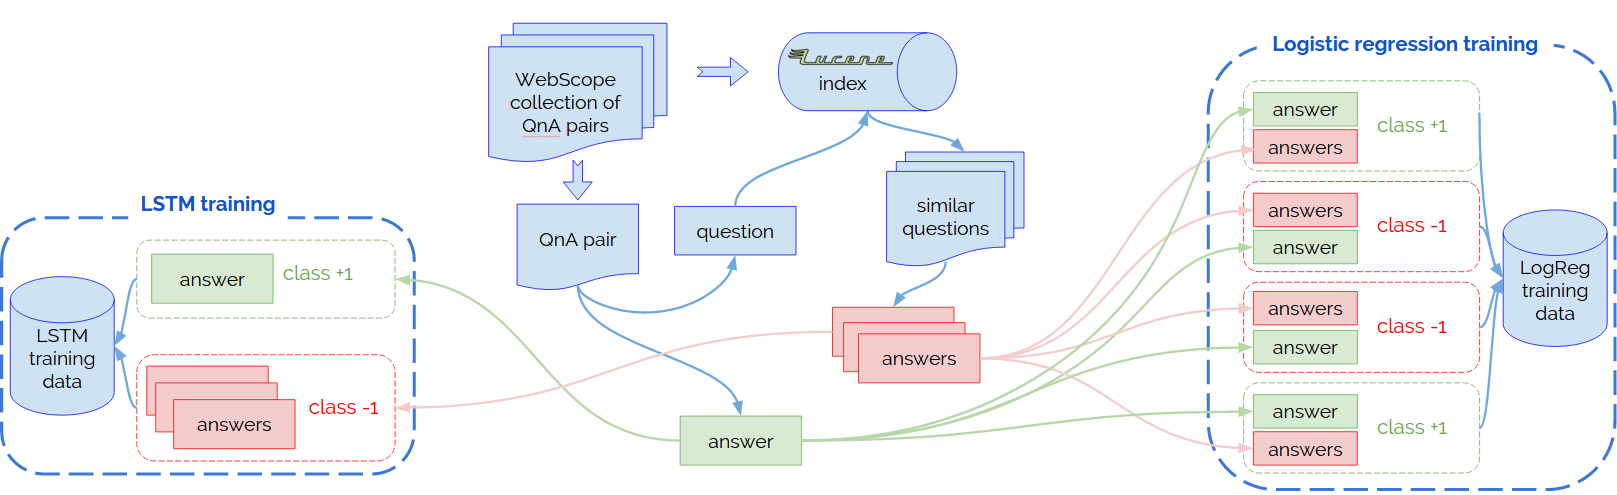
\includegraphics[width=\textwidth]{img/liveqa_model_training}
    \caption{Dataset generation workflow for training logistic regression and LSTM answer ranking models used in EmoryQA system participated in TREC LiveQA 2015.}
    \label{figure:non-factoid:system:model_training}
\end{figure}

\textbf{LSTM model}.
Deep learning models had a huge success in image and speech problems and showed very promising results in natural language processing and question answering, \eg \cite{yu2014deep,WangN15} to name a few.
Long Short-Term Memory (LSTM)~\cite{hochreiter1997long} is a particular architecture of recurrent neural networks that helps with the vanishing gradients problems.
The model reads the question and answer tokens and produces a probability score based on a vector representation of a QnA pair.
Figure~\ref{figure:non-factoid:system:lstm_model} shows the structure of the model.

\begin{figure}[t]
    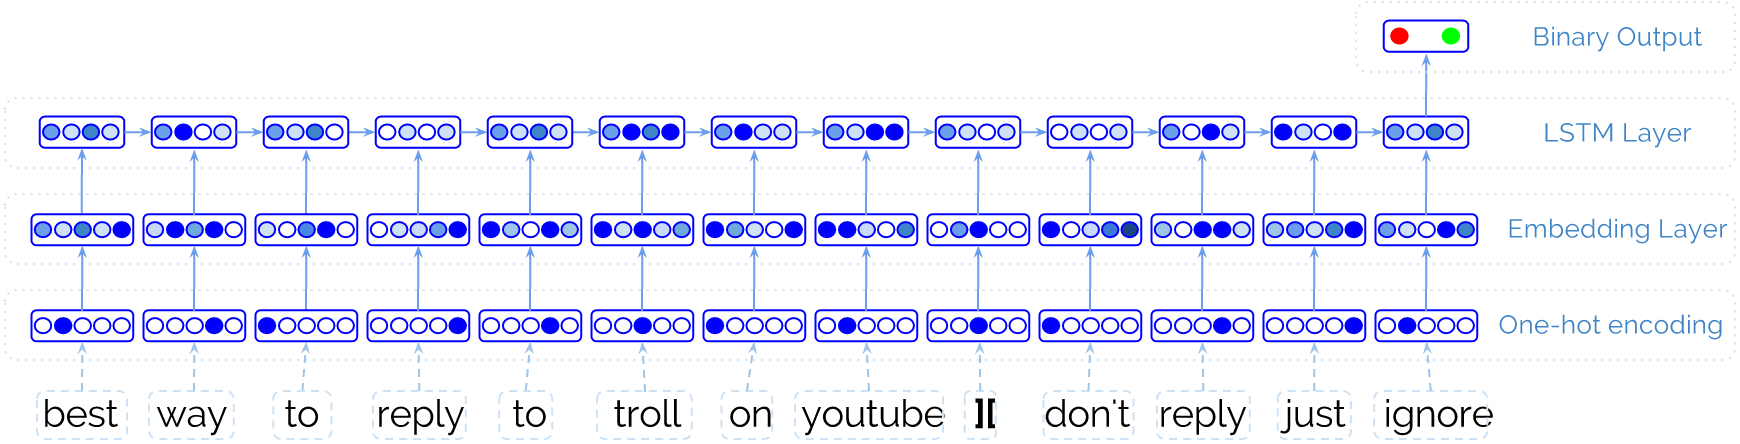
\includegraphics[width=\textwidth]{img/liveqa_qa_lstm}
    \caption{LSTM model for answer scoring used in EmoryQA system, which participated in TREC LiveQA 2015 shared task. The example shows a QnA pair where the question is ``Best way to reply to trolls on youtube?'' and the answer is ``Do not reply, just ignore''.}
    \label{figure:non-factoid:system:lstm_model}
\end{figure}

Question (title with the body) and answer texts are tokenized, punctuation characters are removed and for each token lowercased lemma is taken.
The sequences are limited to 100 elements and concatenated through a sentinel separator character so the model could learn where the question ends and the answer starts.
The hidden state of the model after the whole sequence is processed is used by logistic regression unit to output a probability, that a candidate answers the question well.

The model was trained in a pointwise learning-to-rank fashion~\cite{liu2009learning}, \ie we trained the model to distinguish between the selected best answer and some negative examples.
Random negative examples would be too unrelated to the current question, therefore I chose to use answers to similar questions only.
All QnA pairs were indexed with Lucene\footnote{\href{url}{https://lucene.apache.org/}} and similar questions were retrieved using the built-in BM25 retrieval model.
For each question and correct answer pair from the dataset 10 similar questions were retrieved and the corresponding answers were used as negative examples for training, even though some of them can indeed be relevant to the original question.

The model was implemented using the Keras\footnote{\href{url}{http://keras.io}} library.
I used an embedding and hidden layers of dimension 128 and the vocabulary size of 1M words.
The model was trained using the Adam optimization technique~\cite{kingma2014adam} with mini batches of 200 instances for 100 epochs.

\textbf{Logistic regression model}.
The final model that ranks all answer candidates is a linear L2-regularized logistic regression model.
To train the model we used a different from LSTM model split of QnA pairs from Yahoo! Answers WebScope dataset.
For each question, the corresponding ``best answer'' is taken as the correct one.
To get a sample of negative examples Lucene index is used again and answers to 10 most similar questions are retrieved.
Different from LSTM model training, here I took a pairwise approach for learning-to-rank and generated training examples from pairs of different answers to the same question, where one answer is the correct one.
That is, let the current question be $Q$, its ``correct'' answer $A^*$, and retrieved candidates $A_1, ..., A_n$.
Each candidate is represented with a set of features: $f(Q, A^*)$, $f(Q, A_1)$, ..., $f(Q, A_n)$.
For each $i=1..n$ we create two training instances, i.e. class 1: $\langle A^*, A_i\rangle$ and class -1: $\langle A_i, A^*\rangle$.
Each such instance is represented with pairwise differences of features, e.g. $\langle A^*, A_i\rangle: f_{pair}(Q, \langle A^*, A_i\rangle) = f(Q, A^*) - f(Q, A_i)$.
The trained model is linear, therefore if $w(f(Q, A^*) - f(Q, A_i)) > 0$ then $w f(Q, A^*) > w f(Q, A_i)$ and we can rank candidates by the score produced by the model, i.e. $w f(Q, A_i)$.

% ---------------------------------------
\subsubsection{Learning to rank answers with graded relevance data}
\label{table:non-factoid:system:rel_training}

The approach described in the previous section works well, but the automatic labeling introduces a certain level of noise.
When we have a set of candidate answers with specified graded relevance, as was the case for TREC LiveQA 2016, it is possible to utilize this cleaner data to train an answer ranking model.
Therefore, in TREC LiveQA 2016 for \textit{EmoryQA} we used the listwise approach to learning-to-rank and trained the LambdaMART model~\cite{burges2010ranknet}, which gave the best results on the development set.
This model was trained using the RankLib library\footnote{\href{url}{https://sourceforge.net/p/lemur/wiki/RankLib/}} on the data from the previous year TREC LiveQA task\footnote{\href{url}{https://sites.google.com/site/trecliveqa2016/liveqa-qrels-2015}}.
This data includes 1087 questions with answers provided by the participants, each of which was rated on a scale from 1(bad) to 4(excellent) by professional NIST assessors.



\subsection{Evaluation}
\label{section:non-factoid:system:evaluation}

The experimental evaluation of our \textit{EmoryQA} non-factoid question answering system was done on TREC LiveQA 2015 and 2016 tasks.
The task was to build a live question answering system to respond to user questions, which were sampled from the live stream of questions posted to the Yahoo!~Answers community question answering website by its users.
Each input question consisted of a short question title, body, and category.
A QA system had to provide an answer of 1000 characters or less within a 1 minute period using any available data source.
A reader can refer to \cite{overviewliveqa15,overviewliveqa16} for more details on TREC LiveQA 2015 and 2016 results and analysis.

During the evaluation periods, each system received 1,087 and 1,088 questions correspondingly, and responses were recorded by the organizers.
The answers to the questions were judged by the organizers on a scale:\\
\textbf{4: Excellent} - a significant amount of useful information, fully answers the question.\\
\textbf{3: Good} - partially answers the question.\\
\textbf{2: Fair} - marginally useful information.\\
\textbf{1: Bad} - contains no useful information for the question.\\
\textbf{-2} - the answer is unreadable (only 15 answers from all runs were judged as unreadable).

The official performance metrics used for the tasks are:
\begin{itemize}
\item \textbf{avg-score(0-3)}: average score over all questions, where scores are translated to 0-3 range (1 is subtracted from each judgment). This metric considers ``Bad'', unreadable answers and unanswered questions, as scored 0.
\item \textbf{succ@i+}: success at i+ metrics measures the fraction of answers with score i or greater (i=1..4).
\item \textbf{prec@i+}: precision at i+ measures the number of questions with score i or greater (i=2..4) divided by the number of answered questions.
\end{itemize}

\begin{table}[t]
\centering
\footnotesize
\begin{tabular}[t]
{p{2.5cm}|p{0.8cm}p{1.2cm}p{1.2cm}p{1.2cm}p{1.2cm}p{1.2cm}p{1.2cm}}
& avg score (0-3) & succ@2+ & succ@3+ & succ@4+ & prec@2+ &  prec@3+ & prec@4+ \\
\hline
\multicolumn{8}{c}{Results from TREC LiveQA 2016} \\
\hline
$HUMAN_{qual}$ & 1.561 & 0.655 & 0.530 & 0.375 & 0.855 & 0.692 & 0.490\\
$HUMAN_{speed}$ & 1.440 & 0.656 & 0.482 & 0.302 & 0.784 & 0.576 & 0.362\\
\hline
1. \textit{EmoryCRQA} & 1.260 & 0.620 & 0.421 & 0.220 & 0.644 & 0.438 & 0.228 \\
2. CMU OAQA & 1.155 & 0.561 & 0.395 & 0.199 & 0.596 & 0.420 & 0.212 \\
3. \textbf{EmoryQA} & 1.054 & 0.519 & 0.355 & 0.180 & 0.530 & 0.362 & 0.184 \\
\hline
Avg results & 0.643 & 0.329 & 0.212 & 0.104 & 0.422 & 0.271 & 0.131 \\
\hline
\multicolumn{8}{c}{Results from TREC LiveQA 2015} \\
\hline
1. CMUOAQA &  1.081 & 0.532 & 0.359 & 0.190 & 0.543 & 0.367 & 0.179 \\
2. ecnucs &  0.677 & 0.367 & 0.224 & 0.086 & 0.401 & 0.245 & 0.094\\
3. NUDTMDP1 &  0.670 & 0.353 & 0.210 & 0.107 & 0.369 & 0.219 & 0.111\\
\hline
\multicolumn{8}{c}{...} \\
\hline
7. \textbf{EmoryQA} & 0.608 & 0.332 & 0.190 & 0.086 & 0.408 & 0.233 & 0.106\\
\hline
Avg results & 0.467 & 0.262 & 0.146 & 0.060 & 0.284 & 0.159 & 0.065\\
\end{tabular}
\caption{Top results of the TREC LiveQA 2015 and 2016 shared tasks. EmoryQA is the described fully automatic question answering system. EmoryCRQA is a system with the integrated crowdsourcing module, described in Section~\ref{section:non-factoid:crowdsourcing}.}
\label{table:non-factoid:system:results}
\end{table}

Table~\ref{table:non-factoid:system:results} provides the results of the challenge in 2015 and 2016.
The full results can be found in the official overview reports~\cite{overviewliveqa15,overviewliveqa16}.
As we can see, \textit{EmoryQA} achieves competitive results during both 2015 and 2016 evaluation campaigns.
Improvements made in 2016, \ie additional data sources, listwise learning to rank model, trained on data from previous year task, helped to improve the average answer score by $\approx 70\%$.

Yahoo!~Answers~(qual) and Yahoo!~Answers~(speed) are answers, collected by the organizers from the original questions after a week from the postings.
The \textit{speed} answers are those submitted chronologically first, while \textit{qual} were selected as best answers by the asker, or by Yahoo's quality scoring algorithm.
As we can see, the quality of community answers are still far better, than those of QA systems.
In particular almost $\sim 50\%$ of the questions received a perfect answers from Yahoo!~Answers community, compared to $\sim 22\%$ from the winning system.
However, $\sim 20\%$ of the questions did not receive any response from the community, even though human had the whole week to respond, which stresses an importance of developing automatic approaches even more.

The distribution of answer quality scores and the difference in precision between community and QA systems show, that the later often returns an answer, which is not relevant to the question.
In addition, a quick error analysis also revealed that automatic systems often have trouble recognizing non-relevant passages, which are easily detected by a human even without domain expertise.
The next section describes \textit{EmoryCRQA}, the winning approach from TREC LiveQA 2016, which utilizes crowdsourcing inside a real-time question answering system, and significantly improves performance over the fully automatic approach.


% This plot is using my crowdsourced labels, not official, and it breaks the flow here.
% \begin{figure}
% \centering
% 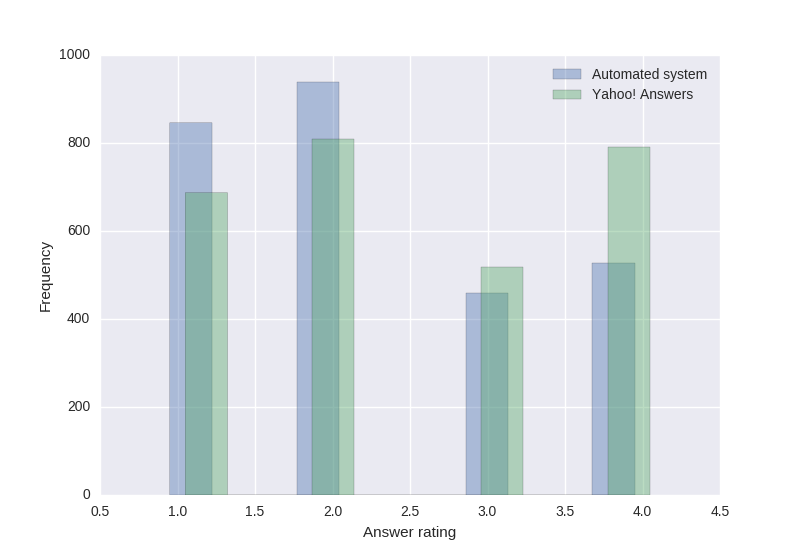
\includegraphics[width=\textwidth]{img/emoryqa_vs_yahoo_scores}
% \caption{Histogram of scores received by EmoryQA and community generated answers}
% \label{figure:non-factoid:system:emoryqa_ya_scores}
% \end{figure}

% On Figure~\ref{figure:non-factoid:system:emoryqa_ya_scores} we can see the distribution of scores received by answers retrieved by EmoryQA system and posted by the community on Yahoo! Answers.

% -=-=-=-=-=-=-=-=-=-=-=-= LiveQA : End -=-=-=-=-=-=-=-=-=-=-=-=-


% ---------------------------------------------------------------------------

\section{CRQA: Crowd-powered Real-time Automatic Question Answering System}
\label{section:non-factoid:crowdsourcing}

As we have seen in the previous section, existing question answering systems are still far from being able to handle every human question.
Answers, submitted by the community users for TREC LiveQA 2016 questions, are $\approx 35\%$ better than the answers from the best performing fully automatic system: CMU OAQA (Figure~\ref{table:non-factoid:system:results}).
One way to overcome the above-mentioned challenges in complex question answering is to develop a hybrid human-computer question answering system, which could consult a crowd of workers in order to generate a good response to the user question.
This section first describes the initial analysis of the feasibility of obtaining different types of feedback from a crowd in real-time.
Then, we present \textit{EmoryCRQA}, a crowd-powered, near real-time automated question answering system for complex informational tasks, that incorporates a crowdsourcing module for augmenting and validating the candidate answers.

More specifically, in this section we answer the following questions:
\begin{enumerate}[itemsep=0em]
\item Can crowdsourcing be used to judge the quality of answers to non-factoid questions under a time limit?
\item Is it possible to use crowdsourcing to collect answers to real user questions under a time limit?
\item How does the quality of crowdsourced answers to non-factoid questions compare to original CQA answers, and to automatic answers from TREC LiveQA systems?
\item Can crowdsourcing be used to improve the performance of a near real-time automated question answering system?
\item What is the relative contribution of candidate answer ratings and answers provided by the workers to the overall question answering performance?
\item What are the trade-offs in performance, cost, and scalability of using crowdsourcing for real-time question answering?
\end{enumerate}

Part of the described results was published at Human-Computer Question Answering workshop at NAACL 2016 conference~\cite{savenkov_crowdsourcing2016a}, and another appeared as a full paper titled ``CRQA: Crowd-powered Real-time Automated Question Answering System'' on HCOMP 2016 conference~\cite{savenkov_crqa2016}.

\subsection{Evaluating crowdsourcing for question answering}
\label{section:non-factoid:crowdsourcing:approach}

In this section I explore two ways crowdsourcing can assist a question answering system that operates in (near) real-time: by providing answer \textit{validation}, which could be used to filter or re-rank the candidate answers, and by \textit{creating} the answer candidates directly.
To test the hypothesis that crowd workers can quickly provide reliable feedback we conducted a series of crowdsourcing experiments using the Amazon Mechanical Turk platform\footnote{\href{url}{http://mturk.com}}.
We used questions from the TREC LiveQA 2015 shared task, along with the systems answers, rated by the NIST assessors\footnote{\href{url}{https://sites.google.com/site/trecliveqa2016/liveqa-qrels-2015}}.
The questions for the task were selected by the organizers from the live stream of questions posted to the Yahoo! Answers CQA platform on the day of the challenge (August 31, 2015).
For these questions, we also crawled their community answers, that were eventually posted on Yahoo!~Answers\footnote{As the answer we took the one selected as the ``Best answer'' by the author of the question or by the community.}.

\subsubsection{Answer validation experiment}
\label{section:non-factoid:crowdsourcing:approach:validation}

To check if crowdsourcing can be used to judge the quality of answers under a time limit, we asked workers to rate answers to a sample of 100 questions using the official TREC rating scale:
\begin{enumerate}[itemsep=0em]
\item Bad --- contains no useful information
\item Fair --- marginally useful information
\item Good --- partially answers the question
\item Excellent --- fully answers the question
\end{enumerate}

\begin{figure}
\centering
\begin{subfigure}[b]{0.49\textwidth}
\centering
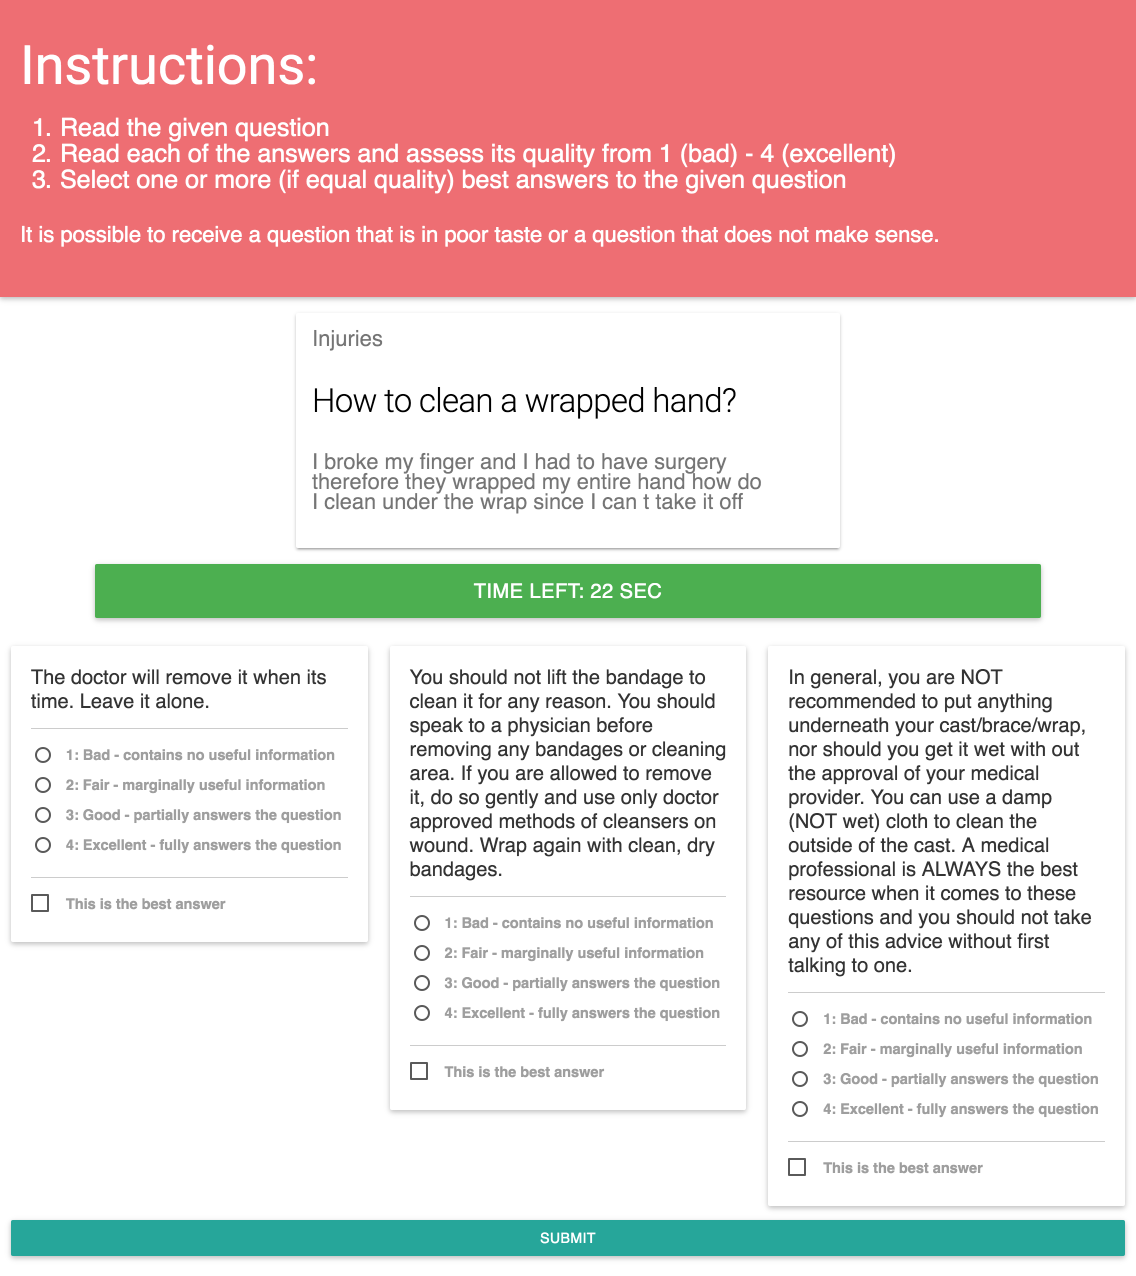
\includegraphics[width=\linewidth]{img/validation_screenshot}
\caption{Answer validation form}
\label{figure:non-factoid:crowdsourcing:interfaces:validation}
\end{subfigure}
\begin{subfigure}[b]{0.49\textwidth}
\centering
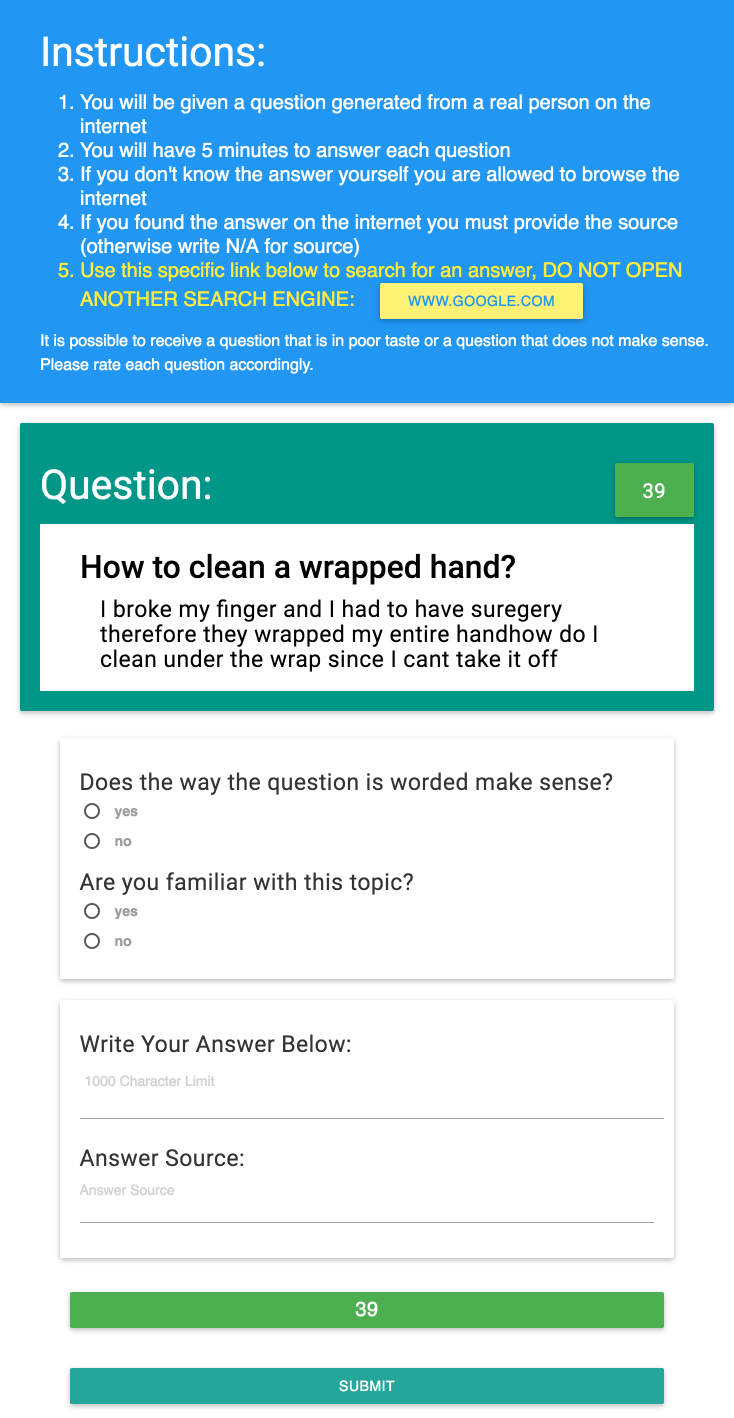
\includegraphics[width=0.9\linewidth]{img/answering_screenshot}
\caption{Answer crowdsourcing form}
\label{figure:non-factoid:crowdsourcing:interfaces:answer}
\end{subfigure}

\caption{User Interface for the answer quality judgment experiment using real-time crowdsourcing.}
\label{figure:non-factoid:crowdsourcing:interfaces}
\end{figure}

We chose to display 3 answers for a question, which were generated by three of the top-10 automatic systems from TREC LiveQA 2015 evaluation \cite{overviewliveqa15}.
To study the effect of time pressure on the quality of judgments we split participants into two groups. One group made their assessments with a 1-minute countdown timer shown to them, while the other could complete the task without worrying about a time limit.
Within each group, we assigned three different workers per question, and the workers were compensated at a rate of \$0.05 per question for this task.

The interface for collecting answer ratings is illustrated in Figure \ref{figure:non-factoid:crowdsourcing:interfaces:validation}\footnote{The screenshots show the final state of the form, as we describe later in this sections fields were unhidden step-by-step for proper timing of reading, answering and validation.}.
On top of the interface, workers were shown the instructions on the task, and question and answers were hidden at this time.
They were instructed to read the question, read the answers, and rate each answer's quality on a scale from 1 (Bad) to 4 (Excellent), and finally, choose a subset of candidates that best answer the question.
Upon clicking a button to indicate that they were done reading the instructions, the question, a 60-second countdown timer and 3 answers to the question appeared on the screen.
At the 15 second mark, the timer color changed from green to red.
In the experiments without time pressure, the timer was hidden, but we still tracked the time it took for the workers to complete the task.

At the end, we collected 6 ratings (3 with and 3 without time pressure) for each of three answers for a sample of 100 questions, which makes it a total of 1800 judgments.
Each answer also has an official NIST assessor rating on the same scale.
Figure \ref{figure:non-factoid:crowdsourcing:score_correlation} shows the correlation between official NIST assessor relevance judgments and ratings provided by our workers.
The Pearson correlation between the scores is $\rho=0.52$.
The distribution of scores shows that official assessors were very strict and assigned many extreme scores of 1 or 4, whereas mechanical turk workers preferred intermediate 2s and 3s.
The results did not show any significant differences between experiments with and without time pressure.
Figure \ref{figure:non-factoid:crowdsourcing:validation_time} shows that even though the median time to rate all three answers is around 22-25 seconds in both experiments, the upper bound is significantly lower in the experiment with the time pressure.

\begin{figure}
    \centering
    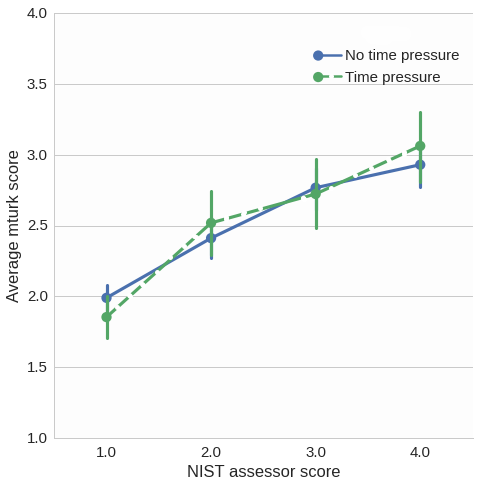
\includegraphics[width=0.5\textwidth]{img/score_correlation}
    \caption{Correlation between NIST assessor scores and crowdsourced ratings with and without time limit on the work time for answers from a sample of 100 questions from TREC LiveQA 2015 task.}
    \label{figure:non-factoid:crowdsourcing:score_correlation}
\end{figure}

\begin{figure}
    \centering
    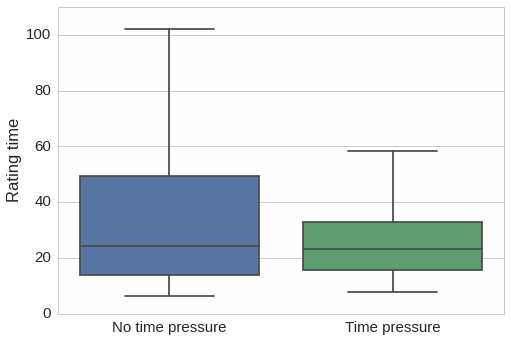
\includegraphics[width=0.5\textwidth]{img/validation_time}
    \caption{Box plot of answer rating time by workers on Amazon Mechanical Turk platform with and without time pressure.}
    \label{figure:non-factoid:crowdsourcing:validation_time}
\end{figure}

Therefore, we conclude that in general we can trust crowdsourced ratings, and on average one minute is enough to judge the quality of three answers to CQA questions.

\subsubsection{Answer generation experiment}
\label{section:non-factoid:crowdsourcing:approach:experiments:generation}

In another experiment, designed to check whether crowd workers can provide an answer to a given question within a limited amount of time, we asked different workers to answer the questions from TREC LiveQA 2015.
We split the workers into two groups and displayed a one-minute countdown timer for one of them.
We left a grace period and let the workers submit their answers after the timer had run out.
The workers received a \$0.10 compensation for each answer.
The form for answer crowdsourcing is shown in Figure \ref{figure:non-factoid:crowdsourcing:interfaces:answer}, and similar to the answer rating form, it starts with a set of instructions for the task.
We let the users browse the internet if they were not familiar with the topic or could not answer the question themselves.
To prevent them from finding the original question on Yahoo! Answers, we included a link to Google search engine with a date filter enabled\footnote{\href{url}{https://www.google.com/webhp?tbs=cdr:1,cd\_max:8/30/2015}}.
Using this link, workers could search the web as it was on 8/30/2015, before TREC LiveQA 2015 questions were posted and therefore workers were in the same conditions as automatic systems on the day of challenge\footnote{The ranking of search results could be different on the day of the challenge and for our workers}.
Initially, the question was hidden for proper accounting of question-reading and answering times.
Upon clicking a button to indicate that they were done reading the instructions, a question appeared along with a button, which needed to be clicked to indicate that they were done reading the question.
After that, the answering form appears, it contained four fields:
\begin{enumerate}[itemsep=0em]
\item Does the question make sense: ``yes'' or ``no'' to see if the question was comprehensible
\item Are you familiar with the topic: A yes or no question to evaluate whether the worker has had prior knowledge regarding the question topic
\item Answer: the field to be used for the user's answer to the given question
\item Source: the source used to find the answer: URL of a webpage or NA if the worker used his own expertise
\end{enumerate}

At the end, we collected 6 answers (3 with and without time pressure) for each of the 1087 LiveQA'15 questions.
Since we have answers from different sources, let's introduce the following notations:
\begin{itemize}[itemsep=0em]
    \item \textit{Yahoo! Answers} - answers eventually posted by users on Yahoo! Answers for the original questions
    \item \textit{Crowd} - answers collected from Mechanical Turk workers without time pressure
    \item \textit{Crowd-time} - answers collected from Mechanical Turk workers with one minute time pressure
    \item \textit{LiveQA winner} - answers from the TREC LiveQA'15 winning system
\end{itemize}

Table \ref{table:non-factoid:crowdsourcing:answer_stats} summarizes some statistics on the answers.
The first thing to notice is that, unlike CQA websites, where some questions are left unanswered, by paying the crowd workers we were able to get at least one answer for all LiveQA questions (after filtering ``No answer'' and ``I do not know'' kind of responses).
The length of the answers, provided by Mechanical turk users is lower, and time pressure forces users to be even more concise.
The majority of workers ($\sim90 \%$) did not use the web search and provided answers based on their experience, opinions and common knowledge.

\begin{table}[h]
\centering
\begin{tabular}{p{3cm}|rrrr}
Statistic & Y!A & mTurk & mTurk-time & LiveQA'15 winner\\
\hline
\% answered & 78.7\% & 100.0\% & 100.0\% & 97.8\% \\
Length (chars) & 354.96 & 190.83 & 126.65 & 790.41 \\
Length (words) & 64.54 & 34.16 & 22.82 & 137.23 \\
\end{tabular}
\caption{Statistics of different types of answers for Yahoo! Answers questions.}
\label{table:non-factoid:crowdsourcing:answer_stats}
\end{table}

\begin{figure}
    \centering
    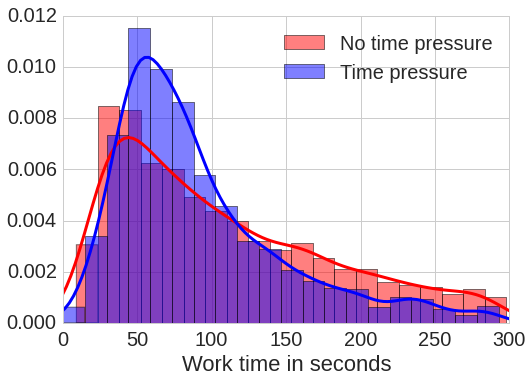
\includegraphics[width=0.6\textwidth]{img/answering_time_distribution}
    \caption{Distribution of answering times for experiments with and without time pressure.}
    \label{figure:non-factoid:crowdsourcing:answering_time_distribution}
\end{figure}

From Figure~\ref{figure:non-factoid:crowdsourcing:answering_time_distribution} we can see that adding time pressure shifts the distribution of answering times\footnote{We had separate timers for reading the instructions, the question, and writing the answer, the inclusion of instruction-reading time is why the total time could be more than 1 minute}.
The tail of longer work times for no time limit experiment becomes thin with time restrictions and the distribution peaks around one minute.

\subsubsection{Answer quality comparison}
\label{section:non-factoid:crowdsourcing:approach:experiments:comparison}

Finally, to compare the quality of the collected answers with the automatic system and CQA responses we pooled together the crowdsourced answers, the answers from the winning and \textit{EmoryQA} systems from LiveQA'15, and the original answers crawled from Yahoo! Answers.
We took a sample of 100 questions and repeated the answer rating experiment on this data.
Each answer was judged by 3 different workers (without time pressure), and their scores were averaged.
Figure~\ref{figure:non-factoid:crowdsourcing:average_score} displays the plot with average score for answers from different sources.
Quite surprisingly the quality of collected answers turned out to be comparable to those of CQA website users.
Average rating of answers produced by the winning TREC LiveQA system is also pretty close to human answers.
Finally, as expected, time pressure had its negative effect on the quality, however, it is still significantly better than the quality of \textit{EmoryQA} answers.

\begin{figure}
    \centering
    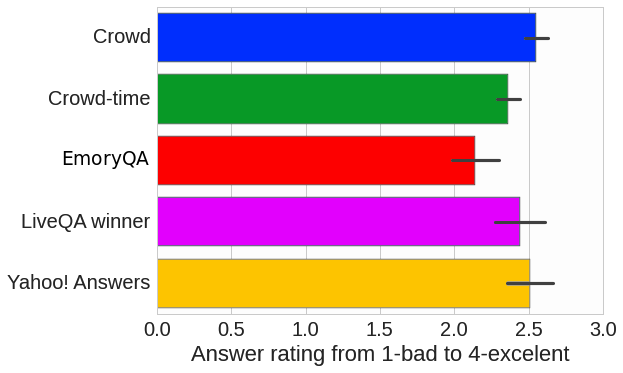
\includegraphics[width=0.6\textwidth]{img/average_score}
    \caption{Average scores of different types of answers to Yahoo! Answers questions.}
    \label{figure:non-factoid:crowdsourcing:average_score}
\end{figure}

\begin{figure}[h]
    \centering
    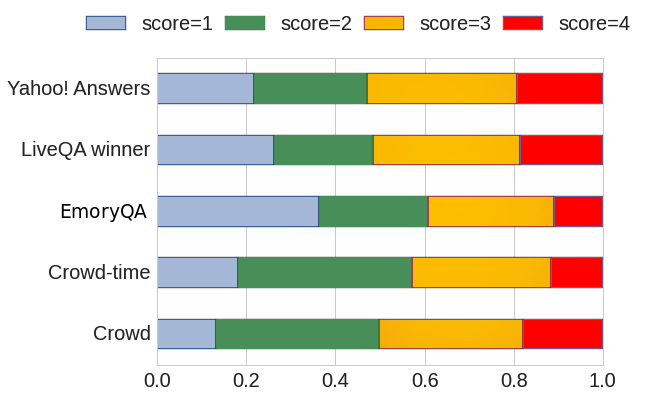
\includegraphics[width=0.6\textwidth]{img/scores_distribution}
    \caption{Distribution of scores for different types of answers to Yahoo! Answers questions.}
    \label{figure:non-factoid:crowdsourcing:scores_distribution}
\end{figure}


Analysis of the score distribution (Figure \ref{figure:non-factoid:crowdsourcing:scores_distribution}) sheds some light on the nature of the problems with automatic and human answers.
The automatic systems generate non-relevant answers ($score=1$) more often than human, either because the systems fail to retrieve relevant information or to distinguish between useful and non-useful answer candidates.
However, by having a larger information store, \eg the Web, automated QA systems can often find a perfect answer ($score=4$), while crowd workers tend to give generally useful, but less perfect responses ($score=2,3$).

Our results suggest that the ``crowd'' can quickly give a reasonable answer to most CQA questions. However, some questions require a certain expertise, which a common crowd worker might not possess.
One idea to tackle this challenge is to design a QA information support system, which a worker can use to help them find additional information.
For example, in our experiment, we let workers use a web search to find answers if they were unfamiliar with the topic; more effective search interfaces may be helpful.

\subsection{System Design}
\label{section:crowdsourcing:approach:crqa}

The findings described in the previous section were used to implement our \textit{EmoryCRQA} system (or simply CRQA), which stands for Crowd-powered Real-time Question Answering.
CRQA integrates a crowdsourcing module into an automated question answering system within an overall learning-to-rank framework for selecting answers to complex questions.
We report extensive experiments of stress-testing the CRQA system, by participating in the TREC LiveQA 2016 evaluation challenge, which provided us with a realistic evaluation setup.

\begin{figure}
    \centering
    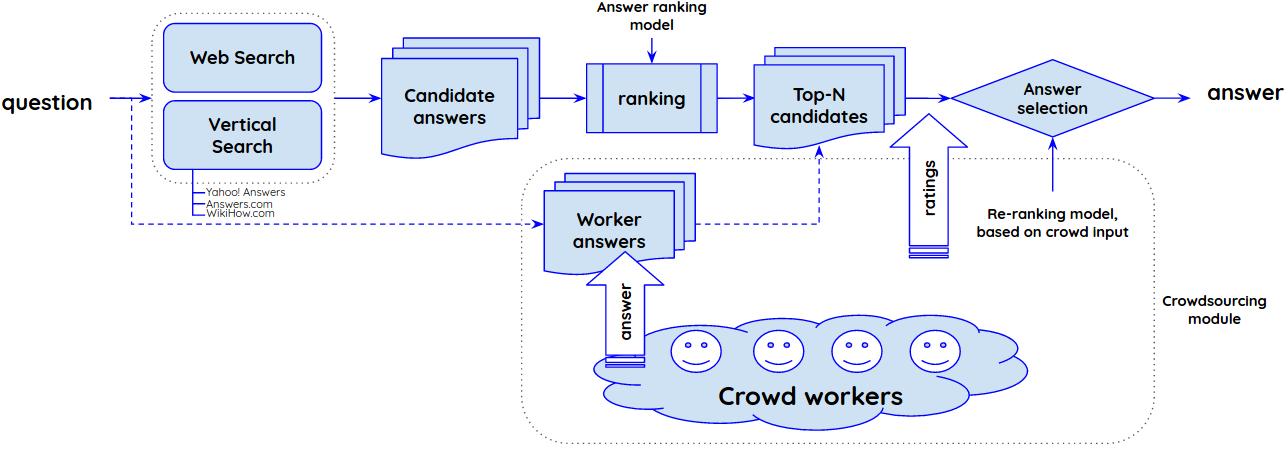
\includegraphics[width=\textwidth]{img/crqa_system}
    \caption{The architecture of our Crowd-powered Real-time Question Answering system, that uses crowdsourcing to augment a list of automatically extracted candidate answers and to rate their quality.}
    \label{figure:non-factoid:crowdsourcing:system}
\end{figure}

The high-level architecture is presented in Figure~\ref{figure:non-factoid:crowdsourcing:system}.
The automated part of the CRQA system is based on EmoryQA system, described in Section~\ref{section:non-factoid:system}.
The crowdsourcing module is designed to overcome two of the most common problems of the automated QA approaches: lack of good candidate answers and ranking errors.
More particularly, CRQA asks crowd workers to provide answers to the given questions if they can, and additionally rate the quality of candidate answers, generated by the automated system.
After the candidate answers are generated, instead of returning the final answer, as EmoryQA does, in CRQA we send the question and top-7 ranked candidates to the crowd workers and wait for the responses.
We chose to give 7 answers based on the average number of rated answers per minute in our preliminary studies.
Figure~\ref{figure:non-factoid:crowdsourcing:crowd_ui} presents the user interface of our crowdsourcing module.

\begin{figure}
    \centering
    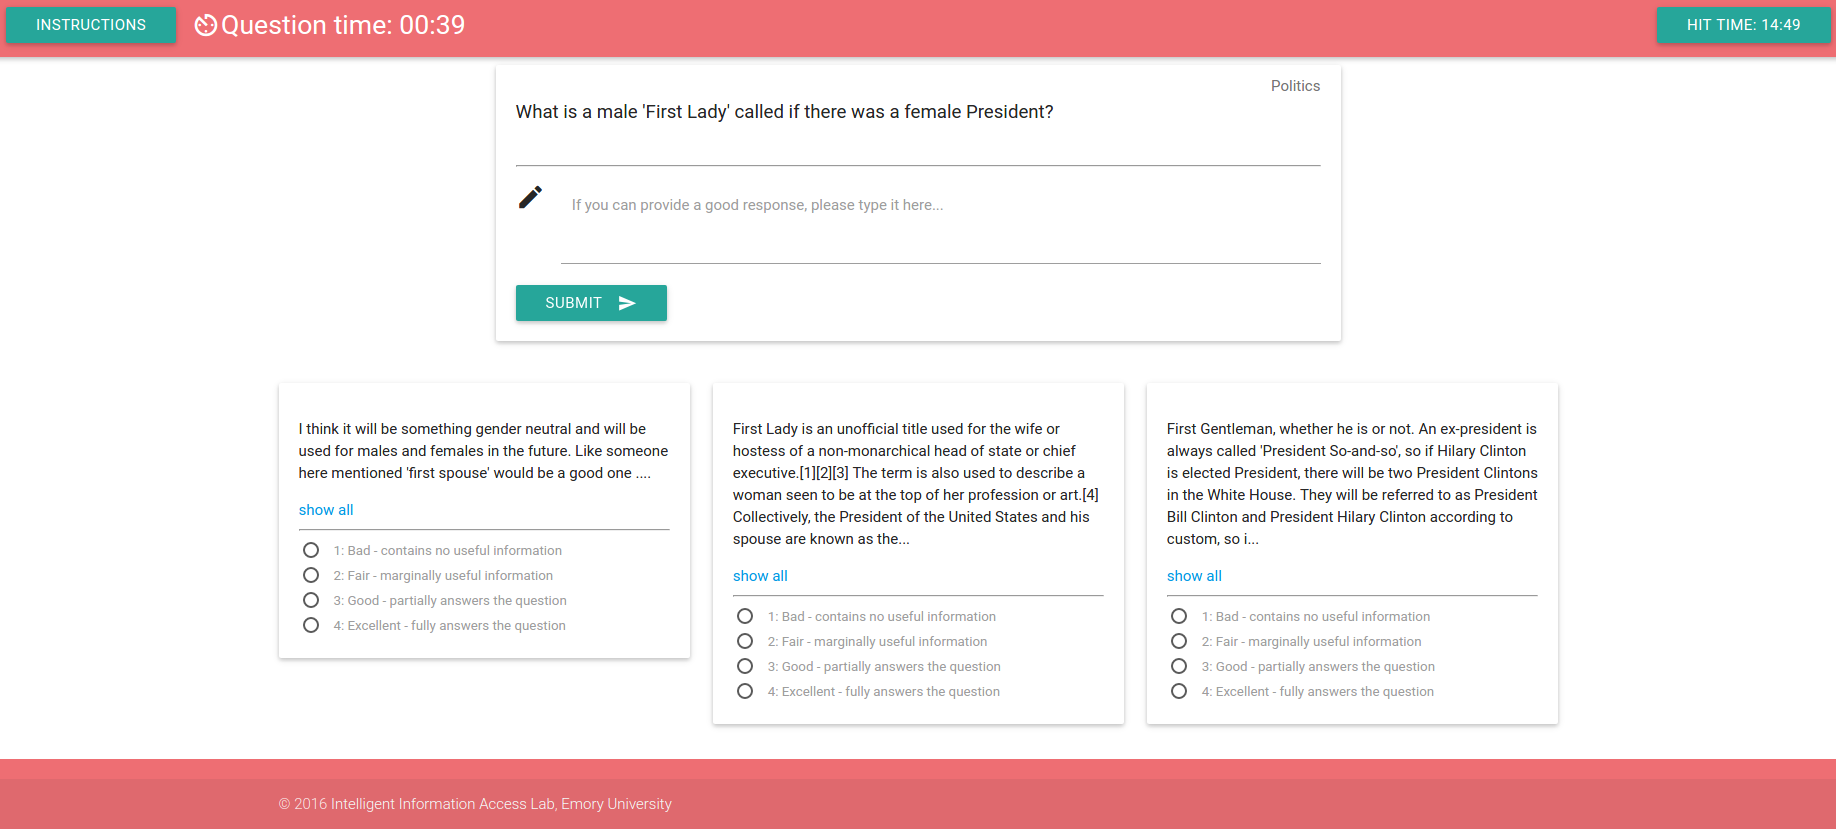
\includegraphics[width=\textwidth]{img/crqa_crowd_ui}
    \caption{User Interface for workers in our Crowd-Powered Question Answering system.}
    \label{figure:non-factoid:crowdsourcing:crowd_ui}
\end{figure}

The overall algorithm for obtaining crowd input for real-time question answering is the following:
\begin{enumerate}[itemsep=0em]
\item When the system receives a question, it is posted to the workers, who will have 50 seconds to provide their input
\item Workers are asked to write an answer if they can provide one (it is optional)
\item Otherwise they are waiting for the answer candidates to arrive
\item When the system is done with generating and ranking candidates it posts top-7 scoring answers to the workers for the rating (which usually leaves $\sim$ 35 seconds for rating)
\item Workers receive a list of answers\footnote{Answers submitted by workers are also sent for ratings to all workers except the author} and rate them until the timer runs off. Each answer is rated on a scale from 1 to 4, using the official TREC LiveQA rating scale:
    \begin{itemize}[itemsep=0em]
    \item 1 --- Bad: contains no useful information
    \item 2 --- Fair: marginally useful information
    \item 3 --- Good: partially answers the question
    \item 4 --- Excellent: fully answers the question
    \end{itemize}
\item The interface displays 3 answers at a time when an answer gets rated, it disappears and its place is taken by another answer from the pool. The interface displays only the first 300 characters of the answer, which was experimentally shown to be enough on average to make a good judgment.
Full answer can be revealed upon clicking the ``show all'' link.
\item When the timer runs off, the question and all the answers disappear, and workers wait for the next question
\end{enumerate}

To hire the workers we used Amazon Mechanical Turk platform\footnote{\href{url}{http://mturk.com}}.
Since the question answering system needs to provide a near real-time response whenever it receives a question, we adapted the ``retainer'' model for real-time crowdsourcing, inspired by the success of this model reported in previous works~\cite{bernstein2011crowds,bigham2010vizwiz}.
Specifically for TREC LiveQA 2016 task, to obtain an even distribution of workers over the 24-hour period, we posted 10 tasks every 15 minutes, and they expired after the next set of tasks became available.
Since not all assignments were accepted by some worker right away, the number of workers for each question varied and could be greater than 10.
When a worker first gets to our crowdsourcing interface, she is shown task instructions (Table~\ref{table:non-factoid:crowdsourcing:crqa:crowd_instructions}) and asked to wait for the questions to arrive.
The workers were paid \$1.00 for the whole 15 minutes task, no matter how many questions they got\footnote{In TREC LiveQA task questions are sent to the systems one by one, therefore there is no concurrency, however, the delays between the questions are possible.}.

\begin{table}[ht]
\centering
\begin{tabular}{p{13cm}}
\textbf{Instructions} \\
\hline
1. This HIT will last exactly 15 minutes\\
2. Your HIT will only be submitted after these 15 minutes\\
3. In this period of time, you will receive some questions, that came from real users on the Internet\\
4. Each question has a time limit after which it will disappear and you will need to want for the next one\\
5. If you know the answer to the question, please type it in the corresponding box\\
6. At some point, several candidate answers will appear at the bottom of the page\\
7. Please rate them on a scale from 1 (bad) to 4 (excellent)\\
8. Do not close the browser or reload the page as this will reset your assignment.\\
\end{tabular}
\caption{EmoryCRQA crowdsourcing task instructions, displayed to the user when she first gets to the task.}
\label{table:non-factoid:crowdsourcing:crqa:crowd_instructions}
\end{table}

The last stage in CRQA is answer re-ranking, which aggregates all the information received from the crowdsourcing and produces the final answer to the question.
The input of the re-ranking module is a set of candidate answers with quality ratings provided by the crowd workers.
Candidates can include the answers posted by the workers, which might also be rated if workers had enough time to do that.
To re-rank the answers we trained a gradient boosting regression trees (GBRT) model~\cite{friedman2002stochastic}.
To build this model we used a training set of questions with answers generated by our system.
The quality of each answer was manually assessed using the official LiveQA scale from 1 (bad) to 4 (excellent).
The features, used for answer re-ranking are listed in Table~\ref{table:non-factoid:crowdsourcing:crqa:reranking_features}.

\begin{table}[ht]
\centering
\begin{tabular}{p{13cm}}
\textbf{Answer-based} \\
\hline
--- The length of the answer \\
--- Source of the answer (Crowd, Web, Yahoo! Answers, Answers.com or WikiHow.com)\\
--- Original rank of the candidate answer or -1 for answers provided by the crowd workers\\
\hline
\textbf{Worker ratings} \\
\hline
--- Number of ratings provided\\
--- Minimum, maximum, median and average ratings\\
\end{tabular}
\caption{The list of features used for answer re-ranking based on crowdsourcing input in EmoryCRQA question answering system.}
\label{table:non-factoid:crowdsourcing:crqa:reranking_features}
\end{table}

CRQA sorts the candidates by the quality score predicted by the model, as returns the top candidate as the final answer.


\subsection{Experiments}
\label{section:non-factoid:crowdsourcing:experiments}

We now describe the experimental setup used to evaluate the performance of CRQA and other methods for near real-time question answering.

The experimental evaluation of our CRQA system was done on the official run of TREC LiveQA 2016 shared task, which happened on May 31, 2016.
All participating systems were running for 24 hours and received questions sampled from the live (real-time) stream of questions, posted by real users to Yahoo! Answers platform.
In total, each system received 1,088 questions, and system responses were recorded by the organizers.

\begin{table}[ht]
\centering
\begin{tabular}{r|l}
Name & Value \\
\hline
Number of questions received & 1088 \\
Number of completed assignments (15 mins each) & 889 \\
Average number of questions per assignment & 11.44 \\
Total cost per question & \$0.81 \\
Average number of answers provided by workers & 1.25 \\
Average number of ratings per answer & 6.25 \\
\end{tabular}
\caption{Aggregate statistics of the crowdsourcing tasks submitted during TREC LiveQA 2016 shared task run.}
\label{table:non-factoid:crowdsourcing:crqa:task_stats}
\end{table}

Overall statistics are provided in Table~\ref{table:non-factoid:crowdsourcing:crqa:task_stats}.
As we can see, on average workers were able to provide at least one answer for each question, and each of the provided answers got 6 ratings.

To perform a full analysis of the system, we used traditional (batch-mode) crowdsourcing to obtain the quality labels for all answer candidates that were given to the workers during the task, as well as the answers provided by the workers.
In addition, on June 2, two days after the TREC LiveQA challenge has completed, we crawled the current answers provided by the community for the questions, used for the task.
All the answers for each question were randomly shuffled and rated on a scale from 1 (bad) to 4 (excellent) by workers hired on Amazon Mechanical Turk.
As we have shown in the previous section, crowdsourced labels correlate well with the official ratings, provided by the professional NIST assessors.
Each answer was labeled by 3 different workers, and we averaged the scores to get the final quality labels for the candidates.

We compared CRQA system against several baselines:
\begin{itemize}
\item \textit{EmoryQA}: automated QA system described in Section~\ref{section:non-factoid:system}.
\item \textit{Re-ranking by score}: a simplified version of the EmoryCRQA re-ranking model, which select the answer with the highest average ratings, provided by the crowd workers.
\item \textit{Yahoo Answers}: traditional, non-real-time community question answering site (Yahoo!~Answers), from which the challenge question originated. The answers were collected two days after the challenge, thus allowing the Yahoo Answers community extra two days to collect the answers through traditional (community-based) crowdsourcing.
\end{itemize}

To evaluate the methods we used the metrics proposed by the organizers of the LiveQA task (Section~\ref{section:non-factoid:system:evaluation}).

\begin{table}[ht]
\centering
\begin{tabular}{p{4.2cm}|rrrrrr}
Method & $\overline{score}$ & $\overline{prec}$ & s@2+ & s@3+ & p@2+ & p@3+ \\
\hline
EmoryQA & 2.321 & 2.357 & 0.697 & 0.297 &  0.708 & 0.302 \\
Re-ranking by score & 2.416 & 2.421 & 0.745 & 0.319 & 0.747 & 0.320  \\
Yahoo! Answers & 2.229 & 2.503 & 0.656 & 0.375 & 0.737 & \textbf{0.421} \\
EmoryCRQA & \textbf{2.550} & \textbf{2.556} & \textbf{0.799} & \textbf{0.402} & \textbf{0.800} & 0.402 \\
\hspace{5mm}worker ratings only & 2.432 & 2.470 & 0.750 & 0.348 & 0.762 & 0.354 \\
\hspace{5mm}worker answers only & 2.459 & 2.463 & 0.759 & 0.354 & 0.760 & 0.355 \\
\end{tabular}
\caption{Evaluation of the baselines and system answers quality based on the ratings of answers obtained via crowdsourcing. The scores are averaged over 100 different 50:50 splits of 1088 questions into the training and test set. The differences between average score and precision of CRQA and the original ranking are significant at p-value $<$ 0.01.}
\label{table:non-factoid:crowdsourcing:crqa:performance}
\end{table}

Table~\ref{table:non-factoid:crowdsourcing:crqa:performance} summarizes the performance of the baselines and our system.
As we can see, the average score and precision of answers generated by CRQA system are higher than the baseline ranking and even community answers on the Yahoo! Answers platform.
However, Yahoo! Answers community answers have a higher percentage of \textit{``4 (excellent)''} scores.
Figure \ref{figure:non-factoid:crowdsourcing:crqa:score_histogram} shows the distribution of scores for the original system ranking, our crowdsourcing system and Yahoo! Answers.
Two peaks on the distribution of scores from Yahoo! Answers community suggest, that there are essentially two kinds of responses: non-useful (\eg spam) or excellent that fully answers the question.
In addition, around 20\% of the questions did not get any answer from the community.
Automatically generated answers, on the contrary, are rarely empty, but on average provide only marginally relevant information, which often does not answer the questions, and therefore rated \textit{``2 (fair)''}.
The introduction of the crowdsourcing module allowed CRQA to cover an additional couple of percents of the questions, for which the automated system was not able to generate any candidates, as well as select better candidates when it was possible using crowd ratings.

\begin{figure}[h]
    \centering
    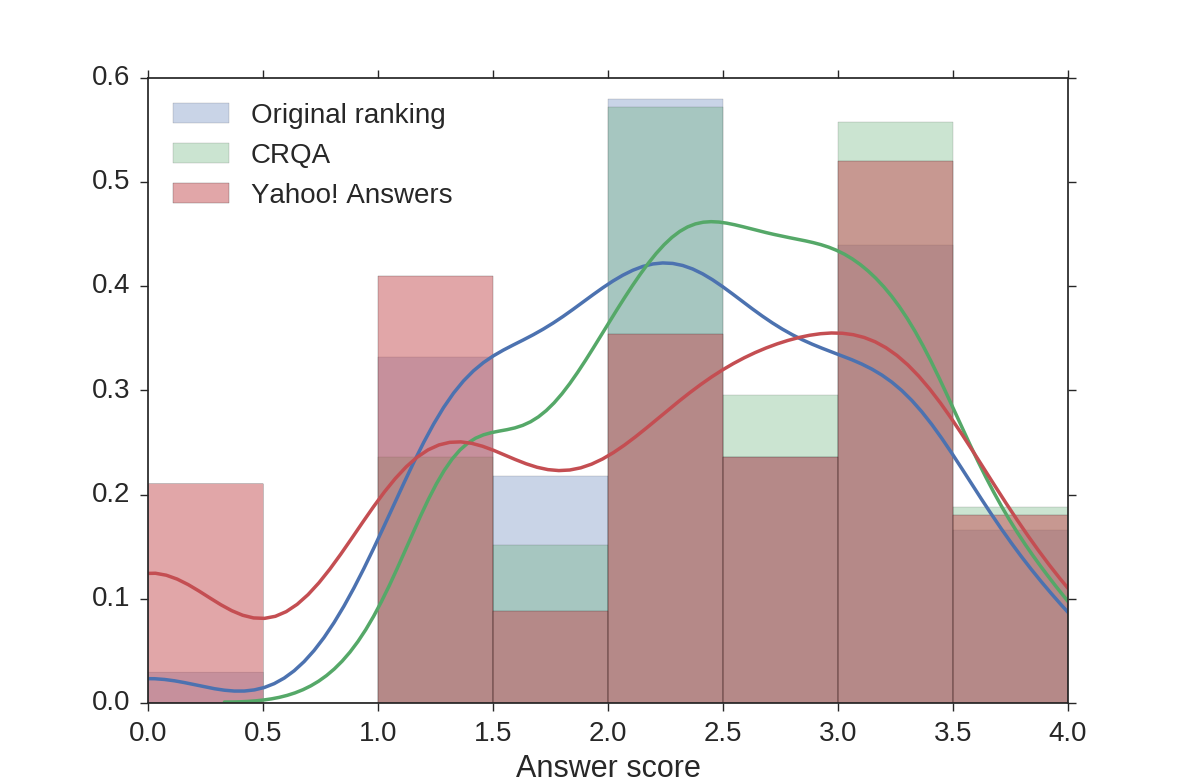
\includegraphics[width=0.75\textwidth]{img/crqa_score_hist}
    \caption{Histogram and kernel density estimation of answer scores for original candidate ranking, CPQA model re-ranking and Yahoo! Answers answers.}
    \label{figure:non-factoid:crowdsourcing:crqa:score_histogram}
\end{figure}

Even though according to the described results our system was able to achieve answer quality comparable to that of the community answers, the official results ~\cite{overviewliveqa16} give slightly different metric values, and demonstrate that there is still a big gap (Table~\ref{section:non-factoid:system:evaluation}).
However, the official scores confirm the effectiveness of crowdsourcing on top of a fully automated QA system.

\subsection{Analysis and Discussion}
\label{section:non-factoid:crowdsourcing:analysis}

In this section, we will analyze some of the results of our experiments and discuss their implications.

\textbf{Worker answers vs ratings}.
First, let's look at the contribution of additional answers and answer ratings provided by the workers.
These two types of contributions are complimentary to each other and attempt to solve different problems.
Table~\ref{table:non-factoid:crowdsourcing:crqa:performance} shows the performance of our question answering system using each of these types of feedback independently.
The results demonstrate that both answers and ratings have a positive effect on the performance.
Even with limited time, workers were able to reliably rate candidate answers, which helped the system to select a better final answer and improve the model precision.
However, this method does not help the system in cases, when it was not able to generate a good candidate in the first place, therefore using ratings only has lower average answer score than using worker generated answers.
By asking the crowd to provide a response if they can answer the question, CRQA covers this gap, which is important as in a real scenario even a fair answer would probably be better for the user than no answer at all.
Of course, given limited time and the fact that a random worker might not possess an expertise required to answer the question, such answers do not always perfectly answer the question.
Table~\ref{table:non-factoid:crowdsourcing:crqa:answer_examples} gives some examples of worker-generated answers with low and high-quality scores.

% To summarize, ratings of answer candidates and worker generated answers both have a similar positive effect on the performance of our question answering system.
% What is more important, the contributions are independent and therefore it is beneficial to use both of them in the final system.

\begin{table}
\centering
\small
\begin{tabular}{p{6cm}|p{5cm}|l}
Question & Answer & Score \\
\hline
 Is Gotu Kola a good herb for mental health? How long does it take to work?? & yes & 1.66\\
 \hline
Can I write any number on line number 5 of a W2?  would like to set up my W2 were I get the most out of my paycheck... & W2 & 1.33\\
 \hline
...i randomly asked my mother why when I lived with you in your home country a man that was our neighbour used to call me his daughter...? & yes & 1.0\\
\hline
\hline
 Is it bad not wanting to visit your family? & It is nt bad. Just be honest with them. They may be upset but they should understand & 3.0 \\
 \hline
Any health concerns with whey protein?... & As long as you use it as directed, there should not be any major problems.  You may want to consult your doctor just in case. & 3.0\\
\hline
Foot pain unable to walk? Hi so today woke with some pain, I am able to put weight on my heel with no problem or pain... & Possible gout in your foot, also possible you may have strained it during the previous day. & 3.0\\
\hline
What is a good remedy/medicine for stomach aches? Specifically ones caused by stress or anxiety? & Chamomile tea should help & 3.66\\
\end{tabular}
\caption{Examples of questions, answers and their quality scores, provided by the crowd workers during TREC LiveQA 2016 shared task.}
\label{table:non-factoid:crowdsourcing:crqa:answer_examples}
\end{table}

\textbf{Selection of answer candidate for rating}.
We have seen that crowd workers are able to provide reliable answer ratings, which can be used to re-rank them and select a better final response.
However, since a system usual has hundreds or thousands of candidate passages, the capacity of crowdsourcing is limited.
We chose to show top-7 answers according to the trained learning-to-rank model, however, the order in which the answers are shown can also have a strong effect on the system performance, because the answers are typically rated one by one in the order they are displayed on the screen.
Our system included two strategies for answer ordering: random or according to their ranking score.
The former strategy provides a uniform coverage for all the answers selected for rating, while the later puts more emphasis on the currently top scoring candidates.
We randomly selected one of the strategies for each user and question.
To analyze the performance of each of the strategies we compute the average score of answers, generated using the corresponding ratings.
The average score for answers generating when candidates are shuffled is 2.508, and it is 2.539 when the candidates are sorted according to their model ranking score.
This suggests, that it is beneficial to allocate more of the worker's attention on the top scoring candidate answers.

\textbf{Cost analysis}.
The results of our experiments clearly demonstrated that crowdsourcing can improve the performance of near real-time question answering system.
The next reasonable question is what is the price of this improvement.
In our study, we paid workers \$1.00 per single 15 minutes task, and each 15 minutes we had 10 assignments, which translates to \$15.00 per 15 minutes.
Overall, our experiment cost \$0.88 per question, and in this section, we will discuss some ideas to reduce this cost.

First, we will study the effect of the number of workers on the performance of our CRQA system.
For this experiment, we randomly sampled a certain percentage of workers and removed all contributions (answers and ratings) of others.
Figure~\ref{figure:non-factoid:crowdsourcing:crqa:nworkers_vs_quality} plots the dependency of the performance of our QA system on the number of workers.

\begin{figure}
  \begin{subfigure}[t]{0.5\textwidth}
    \centering
    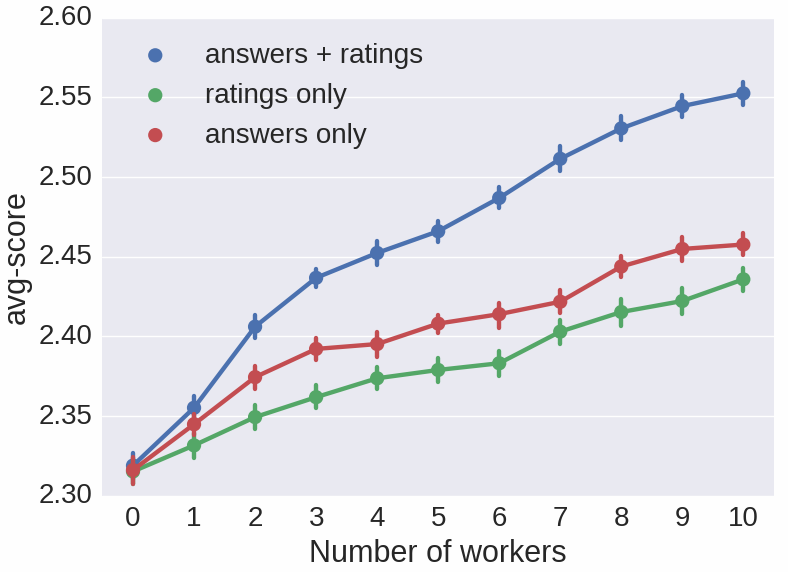
\includegraphics[width=\textwidth]{img/crqa_nworkers_vs_accuracy}
    \caption{avg-score: Average score per question}
    \label{figure:crqa:nworkers_vs_accuracy}
  \end{subfigure}
  \begin{subfigure}[t]{0.5\textwidth}
    \centering
    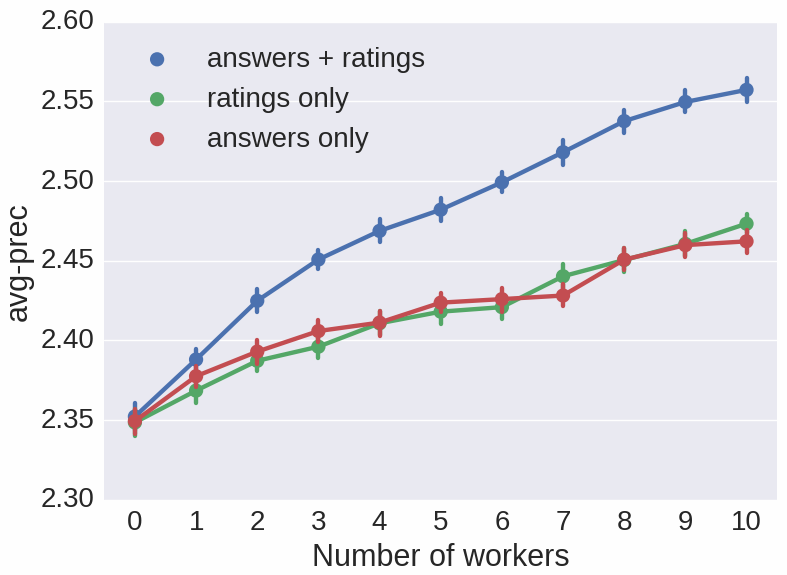
\includegraphics[width=\textwidth]{img/crqa_nworkers_vs_precision}
    \caption{avg-prec: Average score per answer (ignoring non-answered questions)}
    \label{figure:crqa:nworkers_vs_precision}
  \end{subfigure}
    \caption{Plot showing how the quality of the final answer depends on the number of workers per question}
    \label{figure:non-factoid:crowdsourcing:crqa:nworkers_vs_quality}
\end{figure}

Obviously, more workers mean more reliable answer ratings and more answer candidates, which improves the performance of the question answering system.
However, we can observe diminishing returns: the cost per extra gain in performance metrics decreases as the number of workers grows.
Half of the overall performance improvement could be achieved with only 3 workers per question, which would save 70\% of the costs.

An alternative cost-reduction strategy is selective triggering of crowdsourcing, which would only ask for workers feedback for some of the questions.
Such a strategy would be necessary to scale a crowd-powered question answering system to a higher volume of questions.
There are multiple different approaches for such selective crowdsourcing: \eg a system can only ask for crowd contributions if it did not generate enough candidate answers or the predicted quality of the top scoring candidates is low~\cite{carmel2010estimating,he2006query}.
We leave this questions for the future work, as here we focused on the scenario, proposed by the organizers of the TREC LiveQA shared tasks, where questions arrive one by one and it is possible to utilize crowd input for every question.

To summarize, in the explored real-time QA scenario it is possible to reduce the costs of crowdsourcing by reducing the number of workers, although with some performance losses.
Our analysis suggests that paying 30\% of the original cost would give 50\% of the performance improvement.

% The described CRQA implementation is a promising step towards the efficient and close integration of crowd work and automated analysis for real-time question answering.
% It raises many promising issues and opens directions for future work, such as selective crowdsourcing for only the questions deemed ``difficult'' for the automated system; more efficient online learning for obtaining ratings from the crowd and integrating them into the ranking model; and investigating additional features and sources of evidence for improving the joint ranking of the system and crowd input.

\section{Summary}
\label{section:non-factoid:summary}

This chapter described two QA systems aimed at answering a general class of user information needs, often referred to as non-factoid questions.
A fully automatic \textit{EmoryQA} system has information retrieval techniques at its basis, \ie it extracts relevant passages from multiple semi-structured and unstructured sources, represents them with a set of features, uses a learning-to-rank model to sort the candidate answers and selects the top one as the final answer.
The system was experimentally tested on TREC LiveQA 2015 and 2016 shared tasks, achieving very competitive results.
The source code of the system is available at \href{url}{https://github.com/emory-irlab/liveqa}.

The analysis of the TREC LiveQA results revealed that automatic systems often have problems distinguishing between information, that is totally irrelevant and something, that might be of potential use to a user.
As a result, compared to community generated responses, automatic QA systems have a higher fraction of answers, rated ``bad''.
Many of these mistakes can easily be spotted by a human, even without a specific domain expertise.
\textit{EmoryCRQA} extends the fully automatic QA system with a crowdsourcing module, which obtains feedback from a crowd of workers in a form of additional answer candidates and ratings of existing passages, while still operating in near real-time.
Results of TREC LiveQA 2016 task confirmed the effectiveness of crowdsourcing in this scenario.
The analysis presented in Section~\ref{section:non-factoid:crowdsourcing:analysis} shows that both worker contributed answers and ratings make an equal impact on the overall answer quality.
The described CRQA implementation is a promising step towards the efficient and close integration of crowd work and automatic analysis for real-time question answering.

These contributions have laid the groundwork for future research in non-factoid question answering, using various types of semi-structured (QnA pairs), unstructured (web documents) and real-time crowdsourcing data.
Together, the proposed methods enabled substantial performance improvements in answering a wider class of user information needs.